Hash tables generalise the simple notion of direct addressing making effective uise of the ability to examine an arbtrary element of an array in $O(1)$ which we know is not affordable when the key universe is big, because it requires space which is proportional to the size of the universe. 
\subsection{Direct Addressing Table}
Suppose for instance that an application needs a synamic set in which each elemtn has a keu drqwn from the universe $U 0 \{0,1,\ldots m-1\} $ where $m$ is not too large and no towo element share the same key (indiex of the direct addressing table).
A direct addressing table is a indexable structure of size $m$ where each key of the universe has a one to one correspondence to one slot of the table. 
Dictionary operations can be performed as follows:

\begin{algorithm}
\Fn{SEARCH (T,k)}{
	$return T[k]$
 }
 \Fn{INSERT (T,x)}{
	$T[tokey(x)] = x$
 }
 \Fn{DELETE (T,x)}{
	$T[tokey(x)] = NIL$
 }
\caption{DIRECT ADDRESSING OPERATIONS}
\end{algorithm}

	\begin{figure}
	\label{fig:directaddressing}
	\centering
		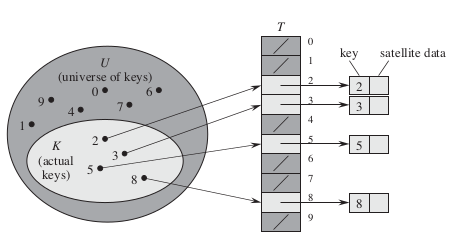
\includegraphics{direct_addressing}
	\end{figure}

where $tokey$ is a function which takes an object $x$ and maps it to an integer in the interval $0\ldots m-1$. Such function is called $hashing function$. 
%---Problem------------
\begin{problem}
\textit{Suppose that a dynamic set S is represented by a direct-address table $T$ of length $m$. Describe a procedure that finds the maximum element of $S$. What is the worst-case performance of your procedure?}.

\begin{solution}
The direct addressing table is not sorted so binary search cannot be used. Only option is a linear scan.
\end{solution}
\end{problem}

Hash tables use addressing with indices as basic idea, but overcome the problem of using large space by using space which is proportional to the number of keys actually stored. The main idea is that we can compute an index from each key to be inserted, in $O(1)$ and use that index as the index of the array location where to store the object. Obviously a because the number of slots is less than the number of possible keys it is possible for two key to be stored at the same location hyelding to a \textit{collision}. There are various effective approach to handle collision which will be describer in the following sections.
In a hash table an element with is stored at slot $h(x)$ where $h$ is an hash function which maps the universe of keys $U$ into slots of the hash table.
\[
h(x): U \mapsto \{0,1,\ldots,m-1\}
\]
with $m$ typically much smaller than $|U|$. The hitch is that (pigeone priciple) two object may be assigned the same slot (they hash to the same slot). This situation is called a \textbf{collision}. There are several tecnquiques to deal with collisions such as 
\begin{enumerate}
\item chaining
\item open addressing
\item linear probing
\item quadratic probing
\item random probing
\end{enumerate}
Of course the best scenario is to avoid collision altogether but since the size of the universe if bigger than the size of the hash table there always exists at least a couple of object which will hash to the same slot. The hash function should, in order to minimize collision as much random as possible (remaining deterministic obviously). The word hash means to mix and it somehow evoke what this function does. It mixes data taken from the object in order to provide a random looking index to be used as an index of the hash table.

\subsection{Collision resolution by chaining}
In chaining, all the elements that hash to the same slot are placed into the same linked-list. The hash table can be viewed, infact, as an array of linked list where each node of the list contains apointer to the object stored.
Dictionary operation can so be performed in average case $O(1)$ as follows:
\begin{algorithm}
\Fn{SEARCH (T,x)}{
	$LIST-SEARCH(T[h(x)]$ 
	\tcc{Worst case - O(n) we will see that average case is much better O(1)}
 }
 \Fn{INSERT (T,x)}{
	$LIST-INSERT-HEAD(T[h(x)],x)$
	\tcc{O(1)}
 }
 \Fn{DELETE (T,x)}{
	$LIST-DELETE(T[h(x)],x)$
	\tcc{O(1) is list are doyhbly linked or O(n) if singly linked}
 }
\caption{Hash table - chaining dictionary operations }
\end{algorithm}

\subsubsection{ANALYSING PERFORMANCE OF HASHING WITH CHAINING}
Given an hash table $T$ we define the \textbf{load factor} ad the ration $\frac{n}{m}$ where $n$ is the actual number of element stored into the hash table and $m$ is the dsize of the table.
